\begin{figure*}[t]
    \centering
    \begin{subfigure}[b]{0.32\textwidth}
    \resizebox{\textwidth}{!}{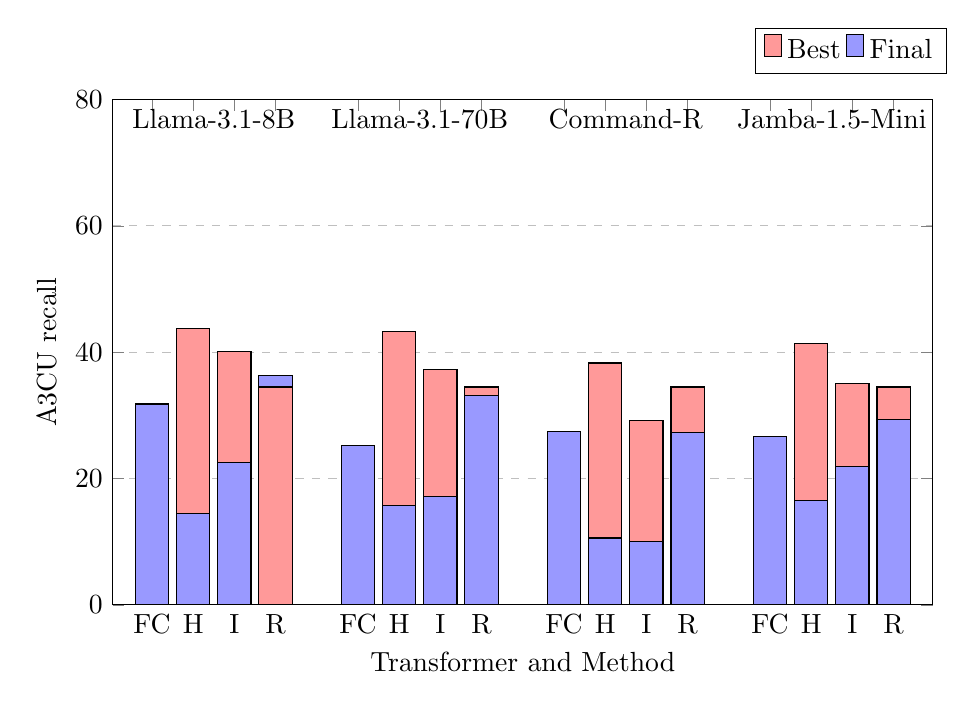
\begin{tikzpicture}
    \begin{axis}[
     width=12cm,
     height=8cm,
     ybar stacked,
     bar width=12pt,
     ylabel={A3CU recall},
     xlabel={Transformer and Method},
     xticklabels={
     FC, H, I, R,
     FC, H, I, R,
     FC, H, I, R,
     FC, H, I, R
     },
     xtick={0,1,2,3,5,6,7,8,10,11,12,13,15,16,17,18},
     x tick label style={anchor=north},
     legend style={at={(0.9,1.05)},anchor=south,legend columns=-1},
     ymajorgrids=true,
     grid style=dashed,
     ymin=0,
     ymax=80,
     enlarge x limits={abs=0.5cm},
    ]
    % Red plot (Best) - only for position 3
    \addplot[fill=red!40] coordinates {
     (0,0) (1,0) (2,0) (3,34.5)
     (5,0) (6,0) (7,0) (8,0)
     (10,0) (11,0) (12,0) (13,0)
     (15,0) (16,0) (17,0) (18,0)
     };
    % Blue plot (Final) - all positions
    \addplot[fill=blue!40] coordinates {
     (0,31.8) (1,14.5) (2,22.6) (3,1.8)
     (5,25.2) (6,15.8) (7,17.2) (8,33.1)
     (10,27.5) (11,10.6) (12,10.1) (13,27.3)
     (15,26.6) (16,16.5) (17,21.9) (18,29.4)
     };
    % Red plot (Best) - all positions except 3
    \addplot[fill=red!40] coordinates {
     (0,0) (1,29.2) (2,17.5) (3,0)
     (5,0) (6,27.5) (7,20.1) (8,1.4)
     (10,0) (11,27.7) (12,19.1) (13,7.2)
     (15,0) (16,24.9) (17,13.1) (18,5.1)
     };
    \legend{Best,Final}
    \node[anchor=north] at (axis cs:1.5,80) {Llama-3.1-8B};
    \node[anchor=north] at (axis cs:6.5,80) {Llama-3.1-70B};
    \node[anchor=north] at (axis cs:11.5,80) {Command-R};
    \node[anchor=north] at (axis cs:16.5,80) {Jamba-1.5-Mini};
    \end{axis}
\end{tikzpicture}}
    \caption{SummHay}
    \label{fig:inf_loss_summhay}
    \end{subfigure}
    % \begin{subfigure}[b]{0.48\textwidth}
    % \resizebox{\textwidth}{!}{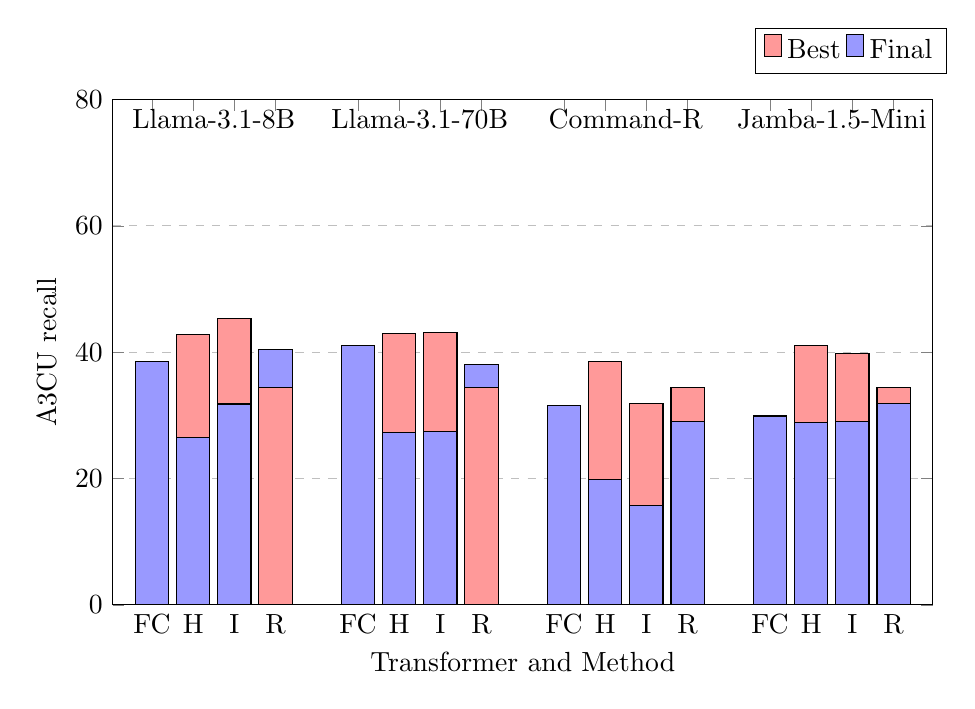
\begin{tikzpicture}
    \begin{axis}[
        width=12cm,
        height=8cm,
        ybar stacked,
        bar width=12pt,
        ylabel={A3CU recall},
        xlabel={Transformer and Method},
        xticklabels={
            FC, H, I, R,
            FC, H, I, R,
            FC, H, I, R,
            FC, H, I, R
        },
        xtick={0,1,2,3,5,6,7,8,10,11,12,13,15,16,17,18},
        x tick label style={anchor=north},
        legend style={at={(0.9,1.05)},anchor=south,legend columns=-1},
        ymajorgrids=true,
        grid style=dashed,
        ymin=0,
        ymax=80,
        enlarge x limits={abs=0.5cm},
    ]
    % Red plot (Best) - only for position 3
    \addplot[fill=red!40] coordinates {
         (0,0) (1,0) (2,0) (3,34.4)
         (5,0) (6,0) (7,0) (8,34.4)
         (10,0) (11,0) (12,0) (13,0)
         (15,0) (16,0) (17,0) (18,0)
     };
    % Blue plot (Final) - all positions
    \addplot[fill=blue!40] coordinates {
        (0,38.5) (1,26.5) (2,31.8) (3,6.0)
        (5,41.0) (6,27.3) (7,27.4) (8,3.6)
        (10,31.5) (11,19.9) (12,15.7) (13,29.0)
        (15,29.9) (16,28.9) (17,29.0) (18,31.9)
    };
    % Red plot (Best) - all positions except 3
    \addplot[fill=red!40] coordinates {
        (0,0) (1,16.3) (2,13.6) (3,0)
        (5,0) (6,15.6) (7,15.7) (8,0)
        (10,0) (11,18.7) (12,16.2) (13,5.4)
        (15,0) (16,12.2) (17,10.8) (18,2.5)
    };
    \legend{Best,Final}
    \node[anchor=north] at (axis cs:1.5,80) {Llama-3.1-8B};
    \node[anchor=north] at (axis cs:6.5,80) {Llama-3.1-70B};
    \node[anchor=north] at (axis cs:11.5,80) {Command-R};
    \node[anchor=north] at (axis cs:16.5,80) {Jamba-1.5-Mini};

    \end{axis}
\end{tikzpicture}}
    % \caption{SummHay (oracle)}
    % \label{fig:inf_loss_summhayoracle}
    % \end{subfigure}
    \begin{subfigure}[b]{0.32\textwidth}
    \resizebox{\textwidth}{!}{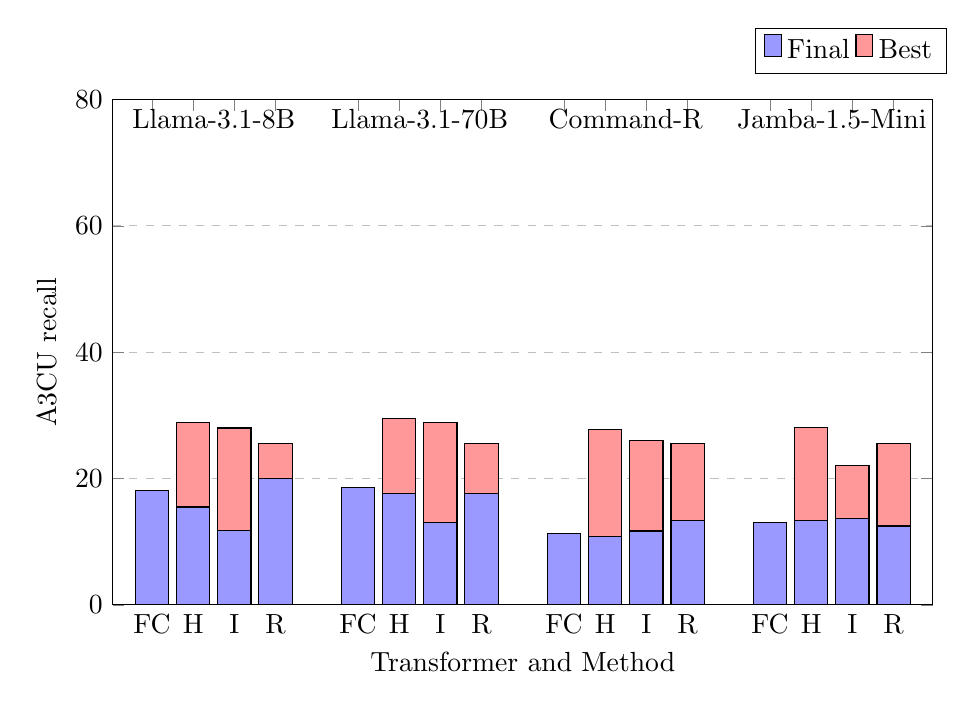
\begin{tikzpicture}
    \begin{axis}[
     width=12cm,
     height=8cm,
     ybar stacked,
     bar width=12pt,
     ylabel={A3CU recall},
     xlabel={Transformer and Method},
     xticklabels={
     FC, H, I, R,
     FC, H, I, R,
     FC, H, I, R,
     FC, H, I, R
     },
     xtick={0,1,2,3,5,6,7,8,10,11,12,13,15,16,17,18},
     x tick label style={anchor=north},
     legend style={at={(0.9,1.05)},anchor=south,legend columns=-1},
     ymajorgrids=true,
     grid style=dashed,
     ymin=0,
     ymax=80,
     enlarge x limits={abs=0.5cm},
    ]
    \addplot[fill=blue!40] coordinates {
     (0,18.1) (1,15.5) (2,11.8) (3,20.0)
     (5,18.6) (6,17.6) (7,13.0) (8,17.6)
     (10,11.3) (11,10.8) (12,11.7) (13,13.3)
     (15,13.1) (16,13.4) (17,13.7) (18,12.5)
     };
    \addplot[fill=red!40] coordinates {
     (0,0) (1,13.4) (2,16.2) (3,5.6)
     (5,0) (6,11.9) (7,15.9) (8,8.0)
     (10,0) (11,17.0) (12,14.3) (13,12.2)
     (15,0) (16,14.7) (17,8.4) (18,13.0)
     };
    \legend{Final, Best}
    \node[anchor=north] at (axis cs:1.5,80) {Llama-3.1-8B};
    \node[anchor=north] at (axis cs:6.5,80) {Llama-3.1-70B};
    \node[anchor=north] at (axis cs:11.5,80) {Command-R};
    \node[anchor=north] at (axis cs:16.5,80) {Jamba-1.5-Mini};
    \end{axis}
\end{tikzpicture}}
    \caption{Background}
    \label{fig:inf_loss_background}
    \end{subfigure}
    \begin{subfigure}[b]{0.32\textwidth}
    \resizebox{\textwidth}{!}{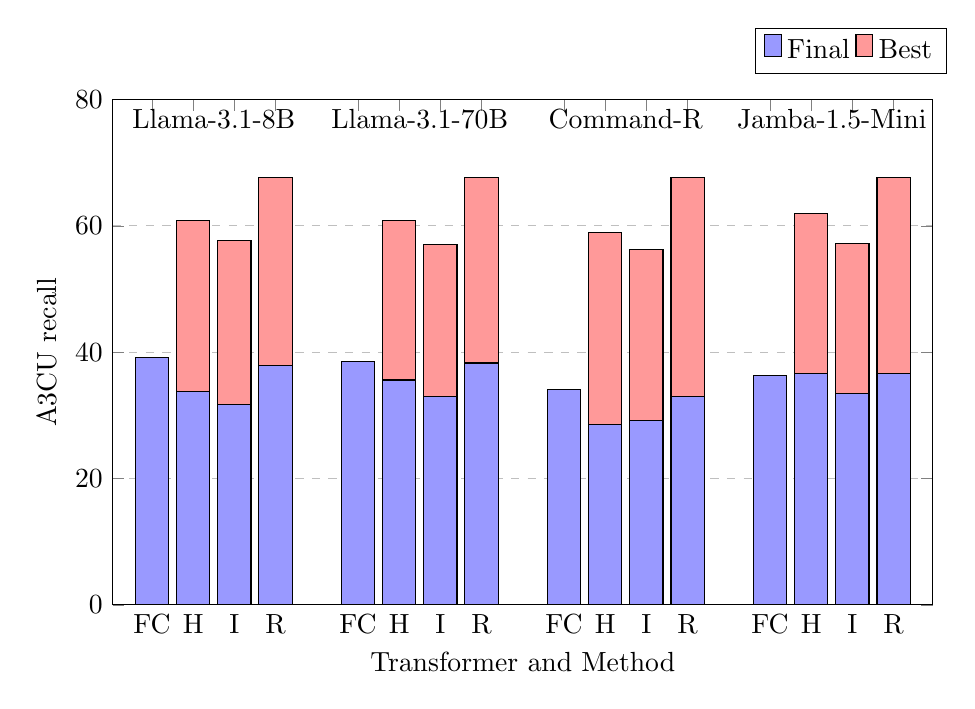
\begin{tikzpicture}
    \begin{axis}[
     width=12cm,
     height=8cm,
     ybar stacked,
     bar width=12pt,
     ylabel={A3CU recall},
     xlabel={Transformer and Method},
     xticklabels={
     FC, H, I, R,
     FC, H, I, R,
     FC, H, I, R,
     FC, H, I, R
     },
     xtick={0,1,2,3,5,6,7,8,10,11,12,13,15,16,17,18},
     x tick label style={anchor=north},
     legend style={at={(0.9,1.05)},anchor=south,legend columns=-1},
     ymajorgrids=true,
     grid style=dashed,
     ymin=0,
     ymax=80,
     enlarge x limits={abs=0.5cm},
    ]
    \addplot[fill=blue!40] coordinates {
     (0,39.1) (1,33.8) (2,31.7) (3,37.9)
     (5,38.6) (6,35.6) (7,33.0) (8,38.3)
     (10,34.1) (11,28.6) (12,29.2) (13,33.0)
     (15,36.3) (16,36.6) (17,33.4) (18,36.6)
     };
    \addplot[fill=red!40] coordinates {
     (0,0) (1,27.0) (2,26.0) (3,29.7)
     (5,0) (6,25.2) (7,24.1) (8,29.3)
     (10,0) (11,30.4) (12,27.0) (13,34.6)
     (15,0) (16,25.4) (17,23.8) (18,31.0)
     };
    \legend{Final, Best}
    \node[anchor=north] at (axis cs:1.5,80) {Llama-3.1-8B};
    \node[anchor=north] at (axis cs:6.5,80) {Llama-3.1-70B};
    \node[anchor=north] at (axis cs:11.5,80) {Command-R};
    \node[anchor=north] at (axis cs:16.5,80) {Jamba-1.5-Mini};
    \end{axis}
\end{tikzpicture}}
    \caption{WCEP}
    \label{fig:inf_loss_wcep}
    \end{subfigure}
    \caption{Salient information retention in the intermediate and final summaries (A3CU \emph{recall}). For each compression method, we report the best recall from the intermediate outputs and the recall of the final summary. (H: hierarchical, I: incremental, R: retrieval, FC: full-context)}
    \label{fig:inf_loss}
\end{figure*}